\section{多场景优化与可解释性}

\subsection{场景定义}

为检验优化框架在不同工程约束下的表现，
定义了4组典型F1赛道工况，
涵盖高速、高下压力、均衡和湿地四种极端设计条件：

\begin{table}[H]
\centering
\caption{四组赛道工况场景定义}
\begin{tabular}{lccccccl}
\toprule
场景 & 速度 (km/h) & 翼角 (°) & DRS & 软约束 & 权重$(w_s, w_e, w_p)$ & 建模意图 \\
\midrule
S1 Monza & 345 (固定) & [20, 29] & 1固定 & 惩罚高阻力 & (0.4, 0.3, 0.3) & 极速赛道，低翼角 \\
S2 Monaco & 300 (固定) & [20, 35] & 0固定 & df$\geq$3000N & (0.5, 0.4, 0.1) & 窄街赛道，高下压力 \\
S3 均衡 & 320 (固定) & [20, 35] & 自由 & 无 & (0.4, 0.4, 0.2) & 中速均衡 \\
S4 湿地 & 290 (固定) & [20, 35] & 0固定 & 无 & (0.6, 0.2, 0.2) & 湿滑路面，稳定优先 \\
\bottomrule
\end{tabular}
\end{table}

S1（Monza高速赛道）模拟意大利Monza赛道的极速特性：
顶速固定于345km/h以匹配赛道设计极速，
翼角搜索范围为20°--29°（工程下限保证气动效率），
DRS强制开启以降低直线阻力。
额外阻力惩罚$0.05 \times (\text{drag}/600)$
引导PSO避开高阻力解。

S2（Monaco高下压力赛道）模拟摩纳哥窄街赛道的特性：
顶速固定于300km/h（匹配赛道弯道密集特征），
翼角搜索范围20°--35°以探索高下压力配置，
硬约束下压力$\geq 3000$N确保产生足够的机械/气动抓地力。
所有场景的翼角下限统一设为20°，
依据真实F1工程约束（前翼小于20°在物理上不可行）。

\subsection{加权标量化多目标适应度函数（v2）}

需要指出，本方法采用加权标量化（Weighted Sum Scalarization）
将多目标问题转化为单目标复合函数进行优化，
属于标量化多目标优化方法的范畴。
严格的种群基Pareto前沿搜索（如NSGA-II、MOPSO）
需要维持非支配解集并直接搜索Pareto前沿，
与本方法的优化机制不同，留给未来工作。

单目标优化的核心问题在于：
当代理模型在大部分参数空间输出接近满分的稳定性时，
优化景观趋于平坦，
PSO退化为随机扰动。
为解决这一问题，
引入多目标加权适应度函数：

\begin{equation}
    F(x) = w_1 \cdot \frac{\text{stability}(x)}{100}
         + w_2 \cdot \tilde{e}(x)
         - w_3 \cdot \tilde{p}(x)
         - \lambda \cdot \sigma(x)
    \label{eq:multiobj}
\end{equation}

其中：
\begin{itemize}
    \item $\tilde{e}(x)$ 为归一化气动效率 $\frac{\text{downforce}}{\text{drag}+\varepsilon}$，
        度量单位阻力产生的下压力；
    \item $\tilde{p}(x)$ 为归一化功率消耗 $\frac{\text{drag} \times \text{speed}}{P_{99}}$，
        反映空气阻力造成的功耗；
    \item $w_1, w_2, w_3$ 为各场景特定的权重向量。
\end{itemize}

需要说明的是，本文各场景的权重向量（如S1的$(0.4,0.3,0.3)$）
由F1赛道工程经验启发设定——
Monza赛道历史上以低阻配置著称（故偏效率），
Monaco赛道以高抓地力需求著称（故偏稳定）。
权重设计的目的是构造具有代表性的多目标偏好场景，
以验证不同工程约束下PSO的多目标权衡求解能力，
而非寻求唯一最优权重配置。
在实际工程应用中，各目标的精确权重可通过
与车队气动工程师的协作或目标空间权衡面上的后验选择来确定。

\subsection{多场景寻优结果}

\begin{figure}[H]
\centering
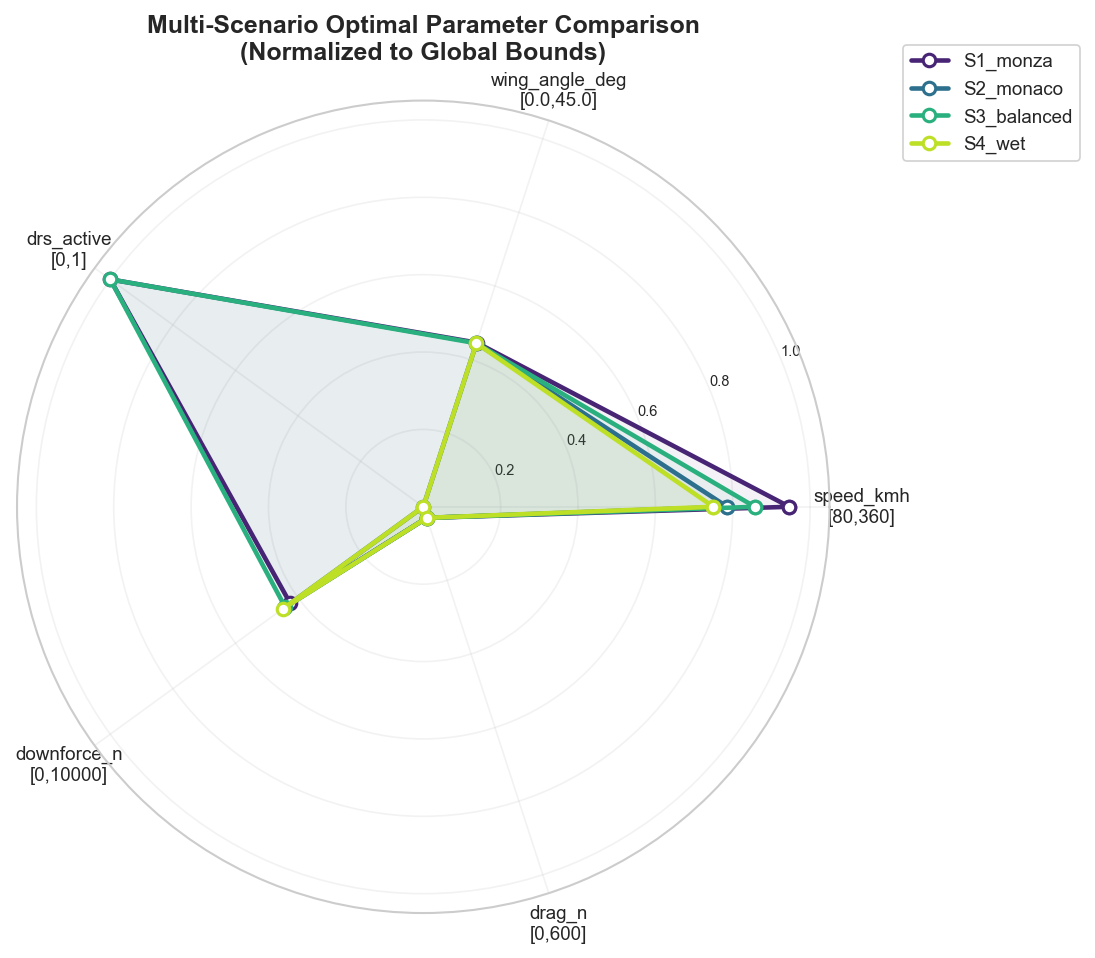
\includegraphics[width=0.78\textwidth]{figures/07_scenario_radar.png}
\caption{四场景最优参数雷达图——归一化到全局搜索边界}
\label{fig:radar}
\end{figure}

图\ref{fig:radar}的雷达图清晰展示了各场景的参数倾向差异：
S1 Monza（红色）在speed轴上偏向高速（归一化值0.71），
wing和drag轴趋于下界（低阻低翼角）；
S2 Monaco（蓝色）在speed轴上趋向下界（低速），
wing轴偏向中等（翼角固定于20°下限）；
S3均衡（绿色）和S4湿地（棕色）的参数分布在诸轴上均偏于保守。

\begin{table}[H]
\centering
\caption{四场景最优参数汇总}
\begin{tabular}{lrrrrrr}
\toprule
场景 & speed & wing & drs & downforce (N) & drag (N) & 复合适应度 \\
\midrule
S1 Monza & 345.0 & 20.1 & 1.0 & 4248.7 & 18.0 & 0.685 \\
S2 Monaco & 300.0 & 20.0 & 0.0 & 4454.2 & 18.0 & 0.894 \\
S3 均衡 & 320.0 & 20.0 & 1.0 & 4411.6 & 18.0 & 0.790 \\
S4 湿地 & 290.0 & 20.0 & 0.0 & 4480.8 & 18.0 & 0.791 \\
\bottomrule
\end{tabular}
\label{tab:scenario_opt}
\end{table}

表\ref{tab:scenario_opt}汇总了各场景最优解的具体值。
关键观察：
\begin{enumerate}
    \item 所有场景的drag均收敛到全局下界18.0N——
        代理模型始终将"低阻力"与"高稳定性"关联，
        这与数据集中downforce\_n$\leftrightarrow$drag\_n的极强正相关（$r=0.895$）一致。
        值得注意的是，Monza（DRS开启）和Monaco（DRS关闭）两场景的drag完全相同，
        表明DRS变量在代理模型中的边际贡献极低：
        SHAP分析显示drs\_active的mean$|$SHAP$|$仅0.01（$<0.1\%$），
        排列重要性中打乱drs\_active后R$^2$下降近乎为零。
        DRS在数据生成器中实质上是一个近乎失效的特征，
        这构成了一项重要的数据诊断发现；
    \item wing\_angle\_deg在所有场景中均集中在20°附近，
        drag在所有场景中均为18.0N——
        表\ref{tab:scenario_opt}中四个场景的权重向量差异显著
        （S1偏效率 vs S4偏稳定），
        但wing和drag的解几乎完全一致。
        这表明多目标景观中stability与efficiency/power的竞争
        尚不足以在wing和drag两个维度产生解的分化——
        退化现象部分延伸至加权多目标空间。
        Landscape Diagnosis（见第9章）将为上述各场景解趋同现象提供统一的因果解释；
    \item 复合适应度在场景间有显著区分：
        S2 Monaco最高（0.894），S1 Monza最低（0.685），
        差异超过23\%，验证了多目标比单目标（区分度仅0.1\%）
        更有效地反映了不同赛道工况的工程偏好。
\end{enumerate}

\subsection{标量化解的权衡分布分析}

由于本方法采用加权标量化（单次PSO运行求解一个确定权重的复合函数），
而非维持非支配解集的种群基Pareto搜索（如NSGA-II），
以下图表中的蓝色折线并非形式化的Pareto前沿，
而是将所有候选解（50粒子$\times$80代）在二维目标空间中的投影
按支配关系筛选后连成的经验权衡前沿面，
用于可视化不同权重配置下的解集分布特征。
需要指出，图中散点来自PSO搜索轨迹（50粒子$\times$80代），
反映的是PSO在当前权重下实际访问的解集分布，
而非目标空间的全量均匀采样。
因此该经验前沿面代表PSO搜索过程中较优解的权衡特征，
不可等同于完整的可行目标空间边界。

\begin{figure}[H]
\centering
\begin{subfigure}{0.48\textwidth}
    \centering
    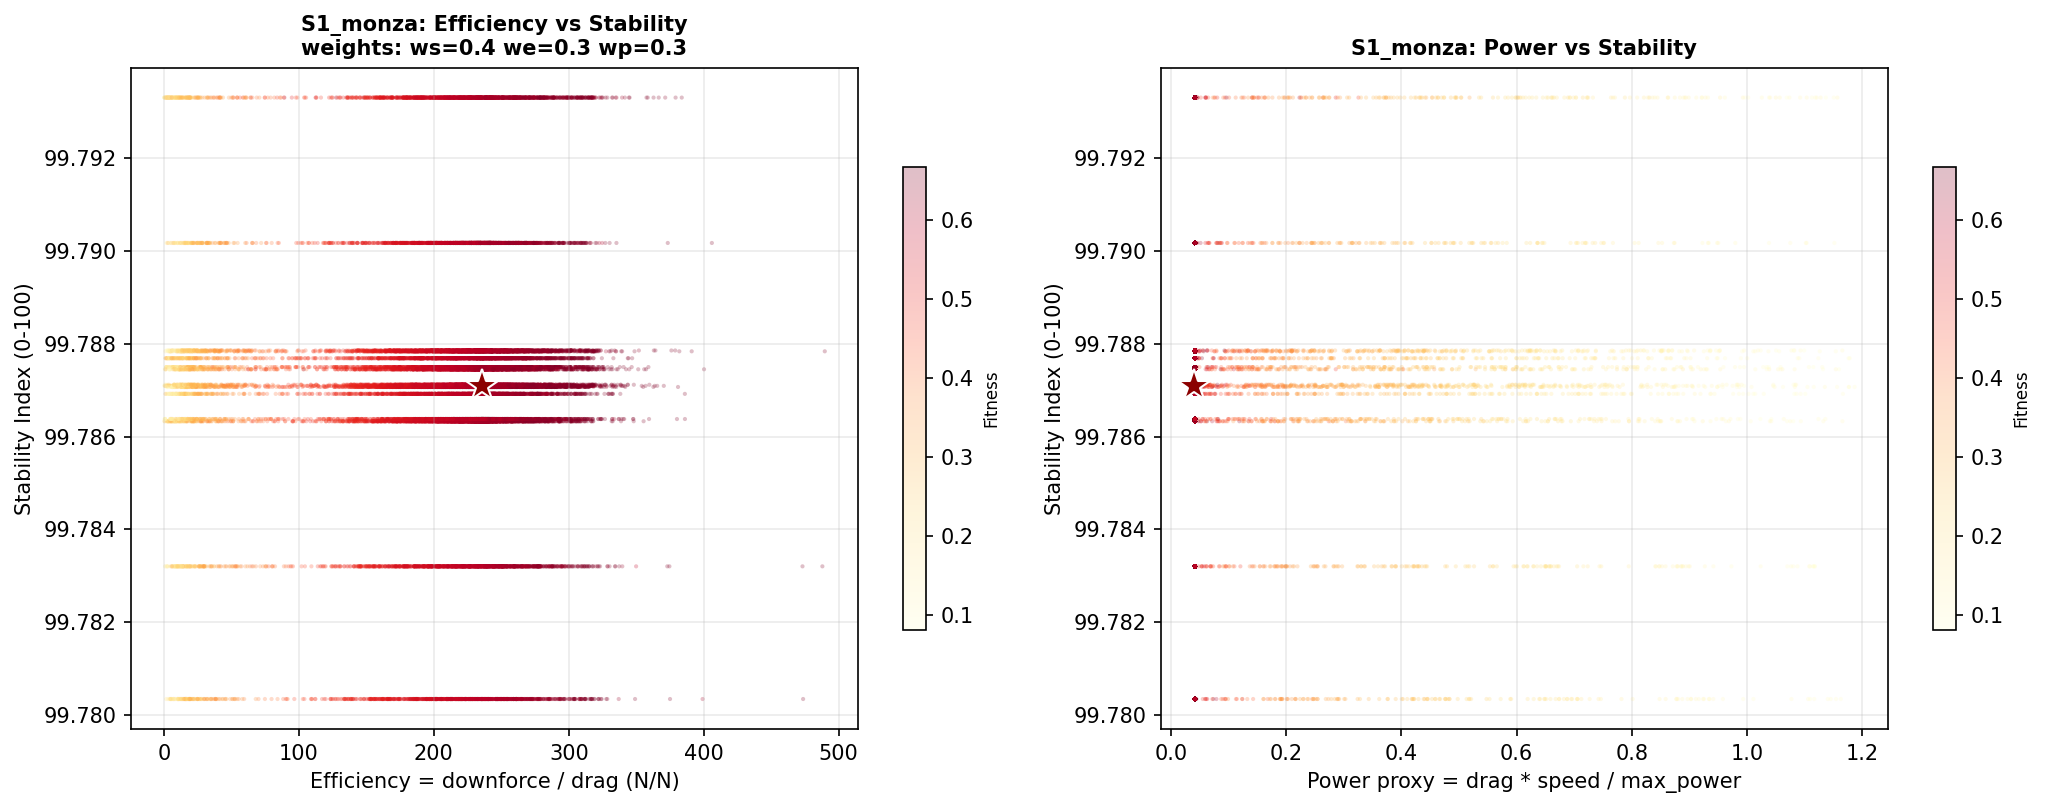
\includegraphics[width=\textwidth]{figures/pareto_frontier_S1_monza.png}
    \caption{S1 Monza（高速低阻优先级）}
\end{subfigure}
\hfill
\begin{subfigure}{0.48\textwidth}
    \centering
    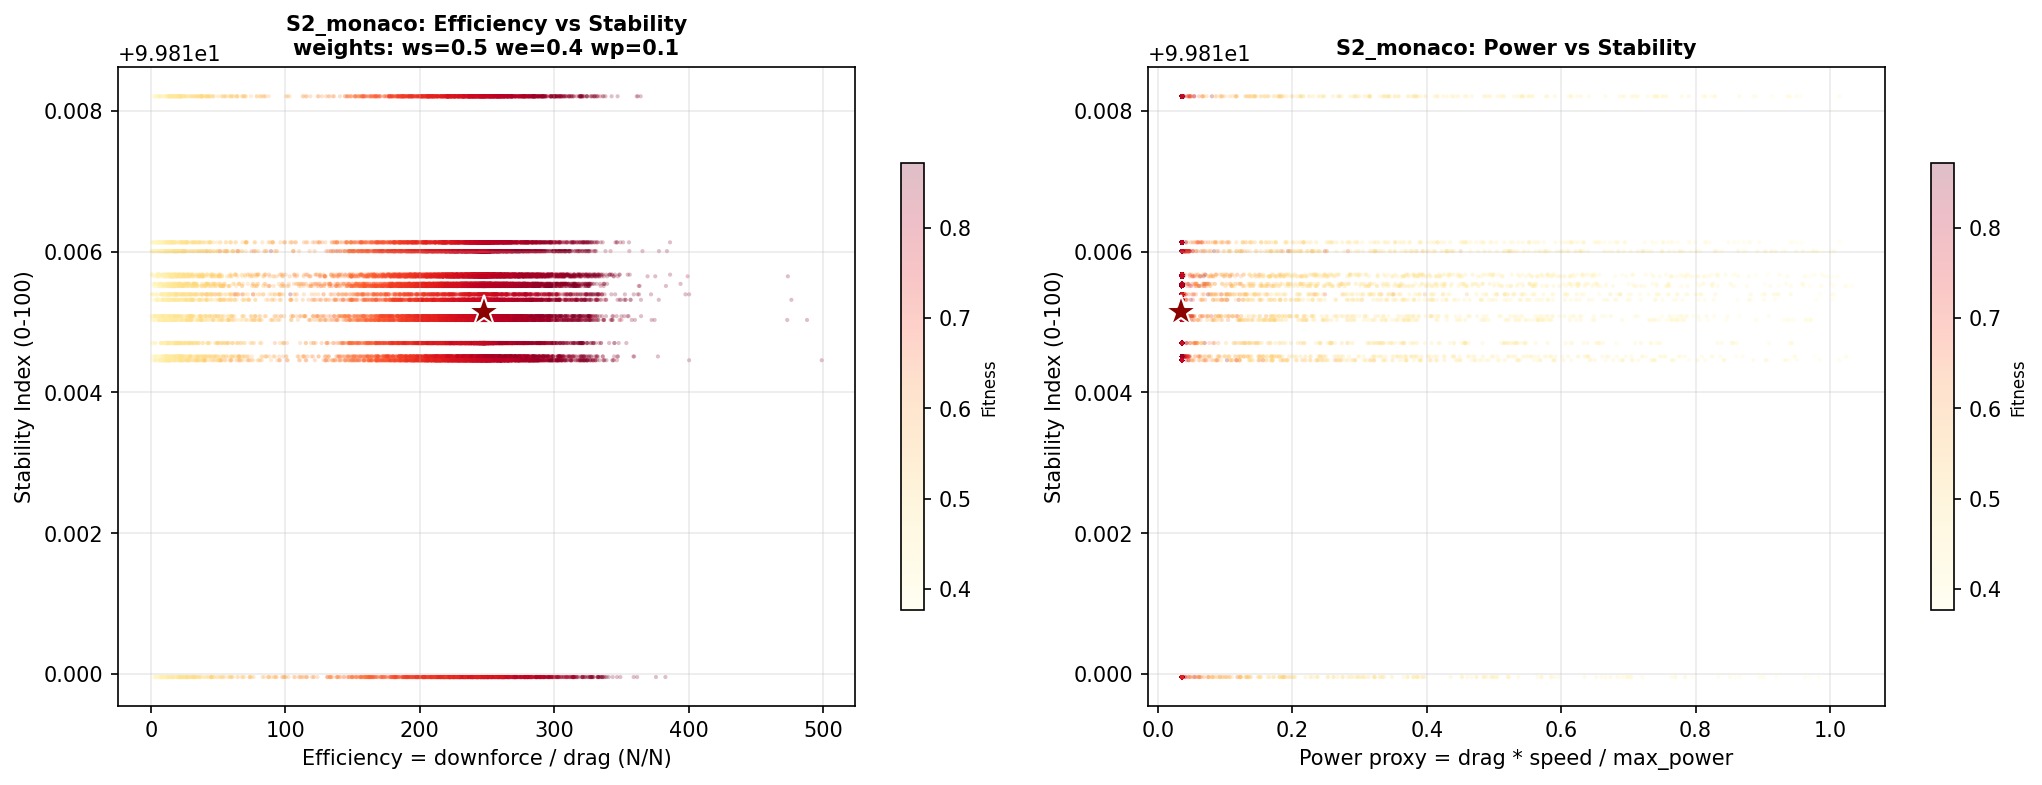
\includegraphics[width=\textwidth]{figures/pareto_frontier_S2_monaco.png}
    \caption{S2 Monaco（高下压力优先级）}
\end{subfigure}
\caption{两场景解集在目标空间中的分布图}
\label{fig:pareto}
\end{figure}

图\ref{fig:pareto}展示了S1和S2所有PSO候选解
在（气动效率, 稳定性）和（功率消耗, 稳定性）目标空间中的投影分布。
每张子图的上半部分为气动效率vs稳定性，
下半部分为功率消耗vs稳定性。
红色大点（★）标记该场景的最优标量化权衡解，
蓝色折线为按支配关系筛选的经验权衡前沿面。
S1的解集分布向高效率侧倾斜，
反映了$w_{\text{efficiency}}=0.3$的权重偏好；
S2则因$w_{\text{stability}}=0.5$的更高权重而在稳定性轴上聚集。

\subsection{场景对比：平行坐标图}

\begin{figure}[H]
\centering
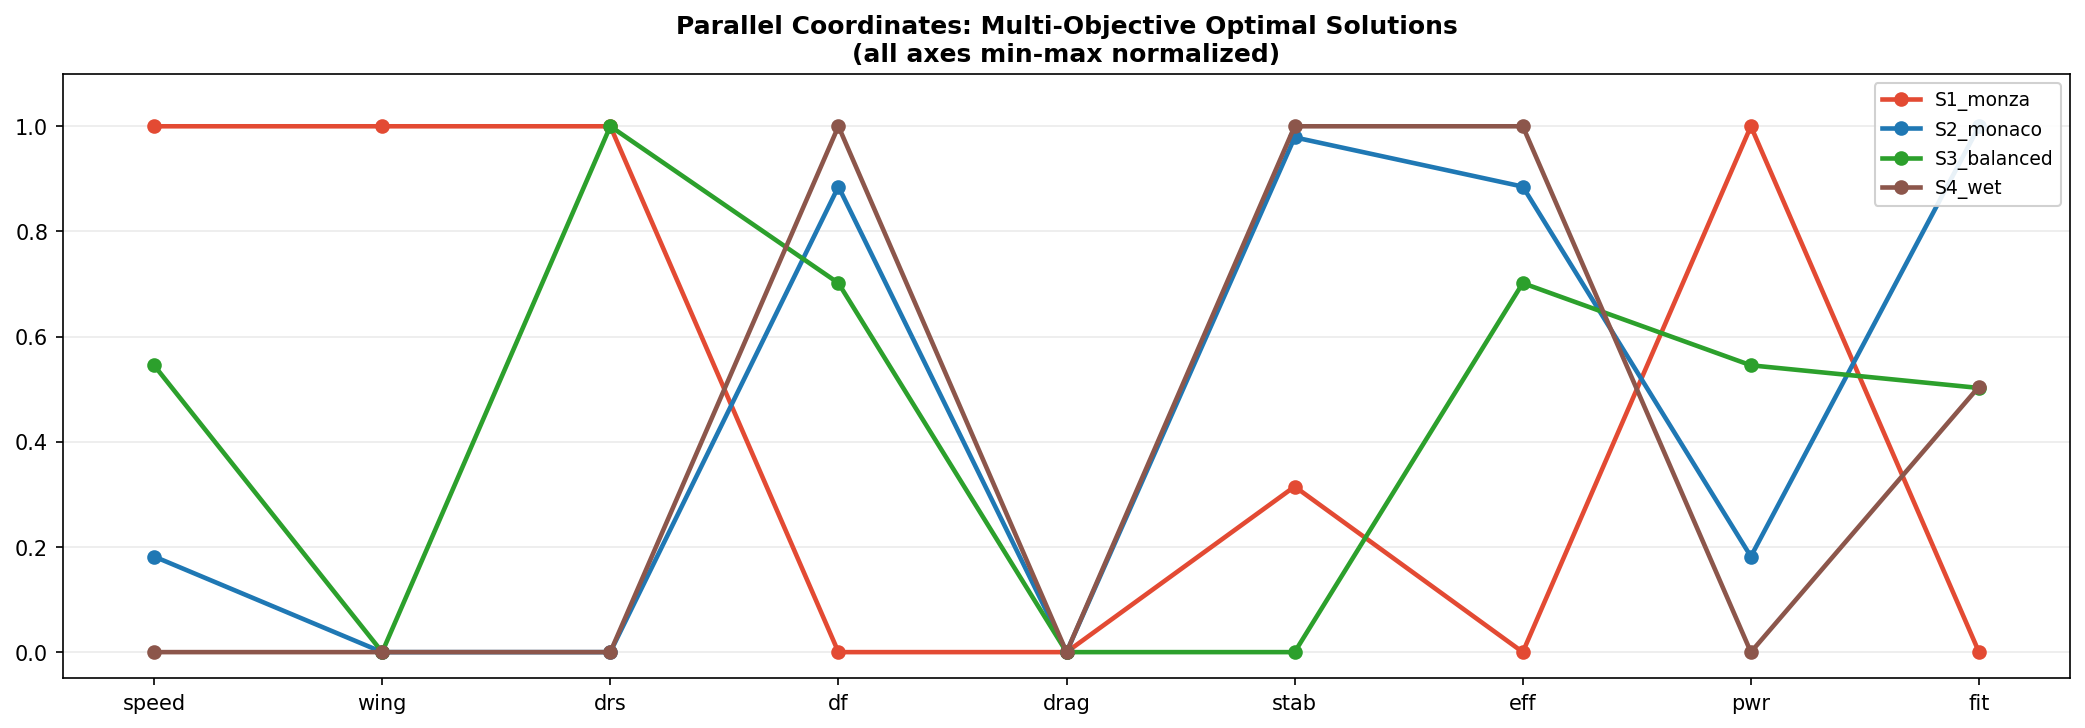
\includegraphics[width=0.85\textwidth]{figures/parallel_coordinates.png}
\caption{四场景最优解的平行坐标对比}
\label{fig:parallel}
\end{figure}

图\ref{fig:parallel}通过9维平行坐标轴展示了各场景最优解的归一化参数差异。
折线在`efficiency`轴和`power`轴上的分离最为显著：
S2 Monaco（蓝色）在`efficiency`轴偏高（高效追求），
S1 Monza（红色）在`power`轴偏低（低功耗偏好）。
`stability`轴上各场景接近——代理模型在该区域输出饱和。

\subsection{SHAP全局可解释性}

\begin{figure}[H]
\centering
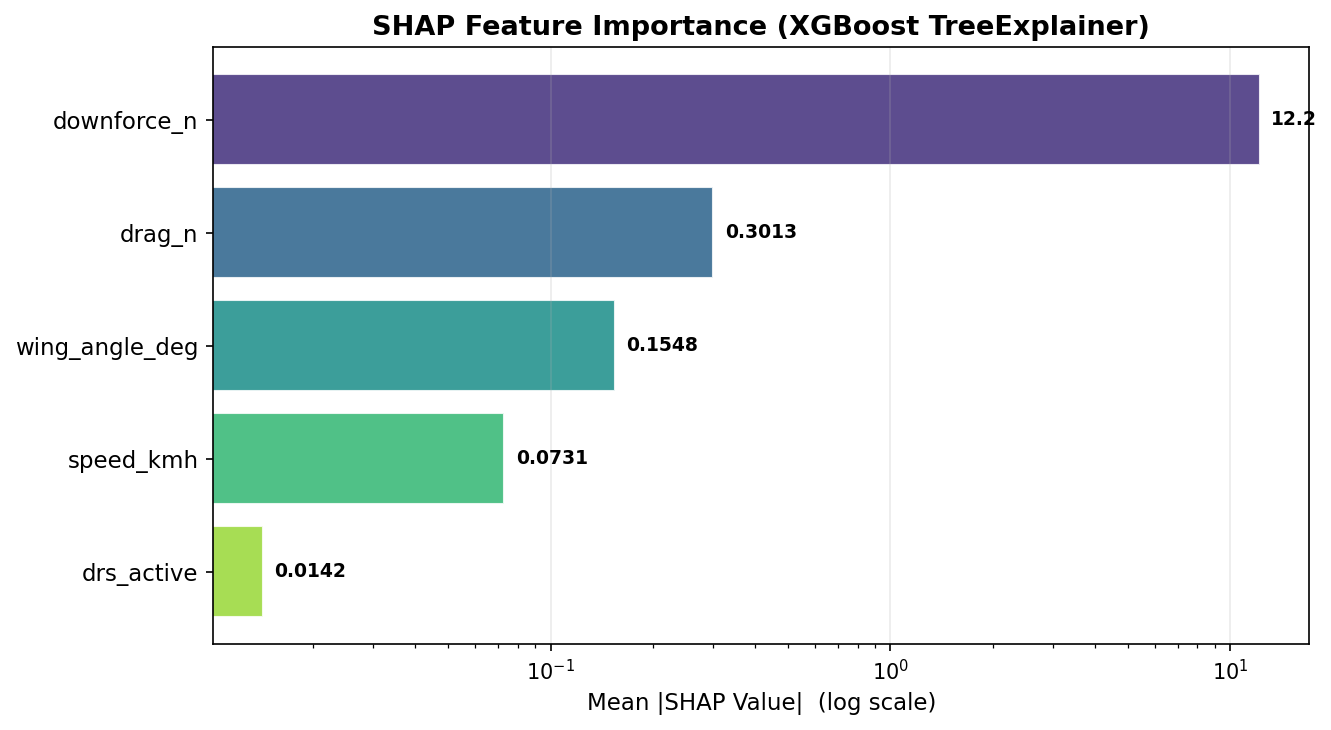
\includegraphics[width=0.78\textwidth]{figures/08_shap_summary.png}
\caption{SHAP全局特征重要性（基于XGBoost）}
\label{fig:shap_global}
\end{figure}

图\ref{fig:shap_global}展示了基于XGBoost的SHAP全局特征重要性。
downforce\_n以mean$|$SHAP$|$ = 12.20的压倒性优势排名第一，
贡献了所有特征中约96\%的预测影响力。
drag\_n（0.30）、wing\_angle\_deg（0.15）、
speed\_kmh（0.07）和drs\_active（0.01）的贡献依次递减。

这一结果揭示了核心的数据驱动事实：
在86\%样本stability$\geq 99$的数据分布下，
代理模型学到的最强信号是"下压力适度即可获满分稳定性"，
其余特征仅提供边际信息增量。

\begin{figure}[H]
\centering
\begin{subfigure}{0.48\textwidth}
    \centering
    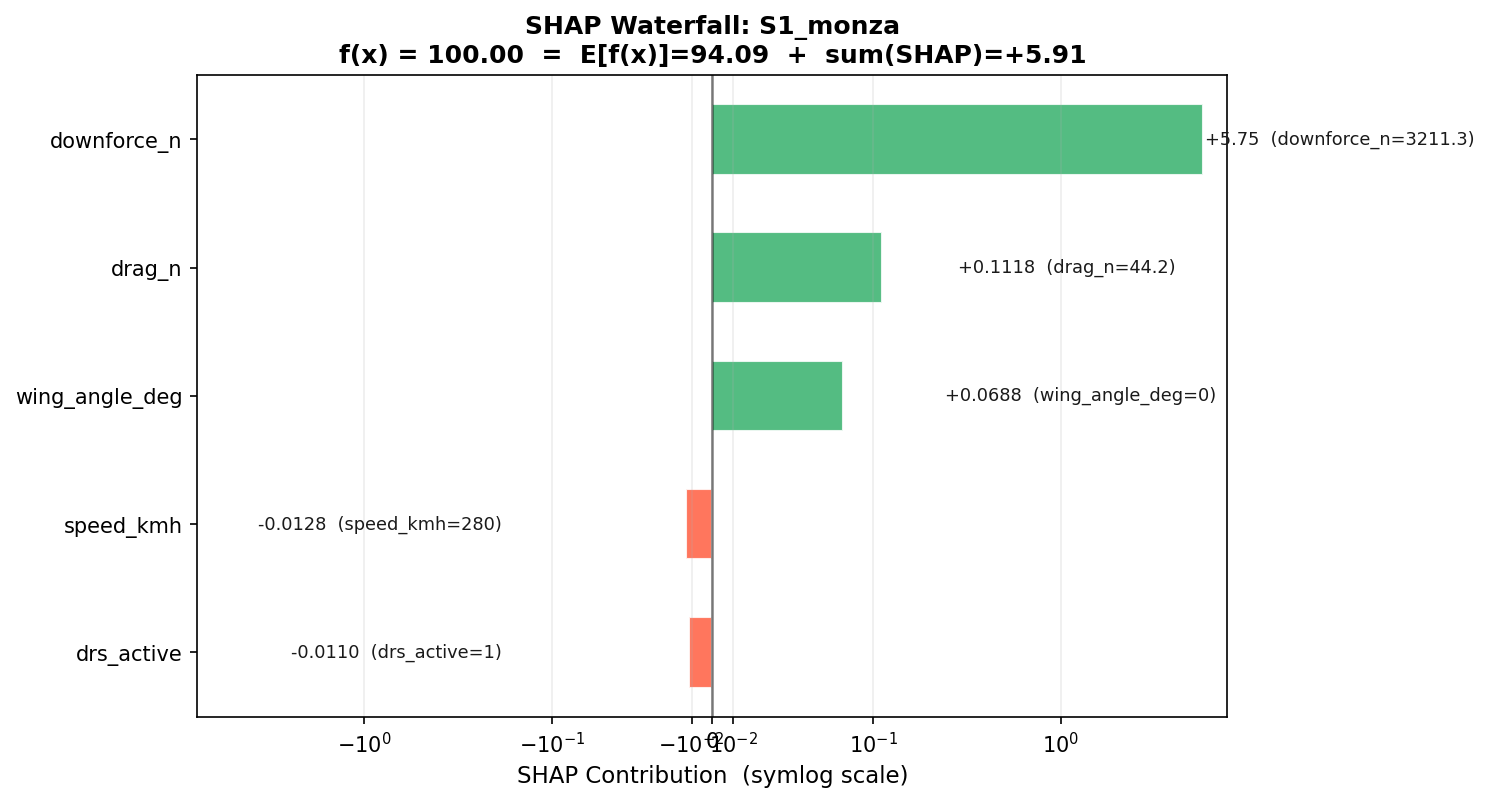
\includegraphics[width=\textwidth]{figures/09_shap_waterfall_S1.png}
    \caption{S1 Monza最优解SHAP瀑布图}
\end{subfigure}
\hfill
\begin{subfigure}{0.48\textwidth}
    \centering
    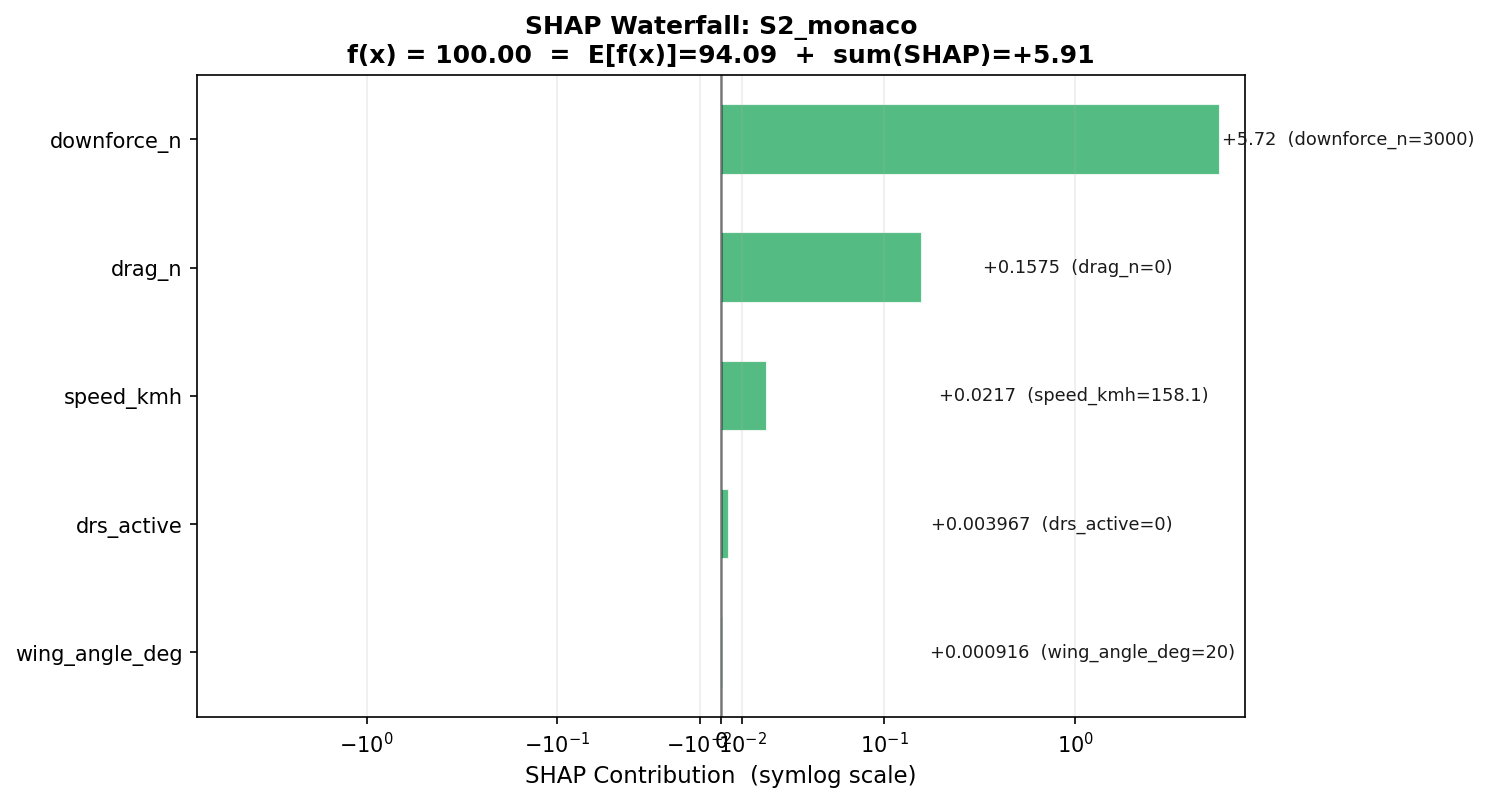
\includegraphics[width=\textwidth]{figures/10_shap_waterfall_S2.png}
    \caption{S2 Monaco最优解SHAP瀑布图}
\end{subfigure}
\caption{两场景最优解的SHAP局部贡献分解}
\label{fig:shap_local}
\end{figure}

图\ref{fig:shap_local}展示了S1和S2最优解的SHAP局部贡献瀑布图。
两个场景的SHAP贡献结构几乎一致：
downforce\_n贡献$+5.75$（推高预测），
drag\_n贡献$+0.11$，其余特征贡献可忽略。
所有场景的最终预测$\hat{y}$均达到100.00（满分），
验证了代理模型在高稳定性区域的输出饱和特征。

\subsection{排列重要性验证}

排列重要性（Permutation Importance）作为SHAP的独立验证，
通过在测试集上随机打乱各特征列后测量R$^2$下降量来评估特征重要性。

\begin{table}[H]
\centering
\caption{排列重要性结果}
\begin{tabular}{lrr}
\toprule
特征 & R$^2$下降量 & 标准差 \\
\midrule
downforce\_n & \textbf{1.879} & 0.012 \\
drag\_n & 0.0014 & 0.00002 \\
wing\_angle\_deg & 0.0004 & 0.00001 \\
speed\_kmh & 0.0002 & 0.000003 \\
drs\_active & 0.00001 & 0.000000 \\
\bottomrule
\end{tabular}
\end{table}

排列重要性与SHAP结论完全一致：
打乱downforce\_n后R$^2$下降1.88（模型近乎瘫痪），
而打乱其余特征对模型性能几乎无影响。
SHAP和排列重要性两种独立方法的相互印证，
增强了"当前特征表达下downforce\_n呈现压倒性贡献"这一结论的可信度。
需要指出，downforce\_n与drag\_n之间存在强共线性（$r=0.895$），
在共线特征场景下，SHAP和排列重要性可能将部分drag\_n的预测信息归因至downforce\_n。
因此上述解释贡献分布应理解为该特定特征空间下的相对重要性，
而非各特征在物理因果层面的独立贡献。

\subsection{约束灵敏度分析}

\begin{figure}[H]
\centering
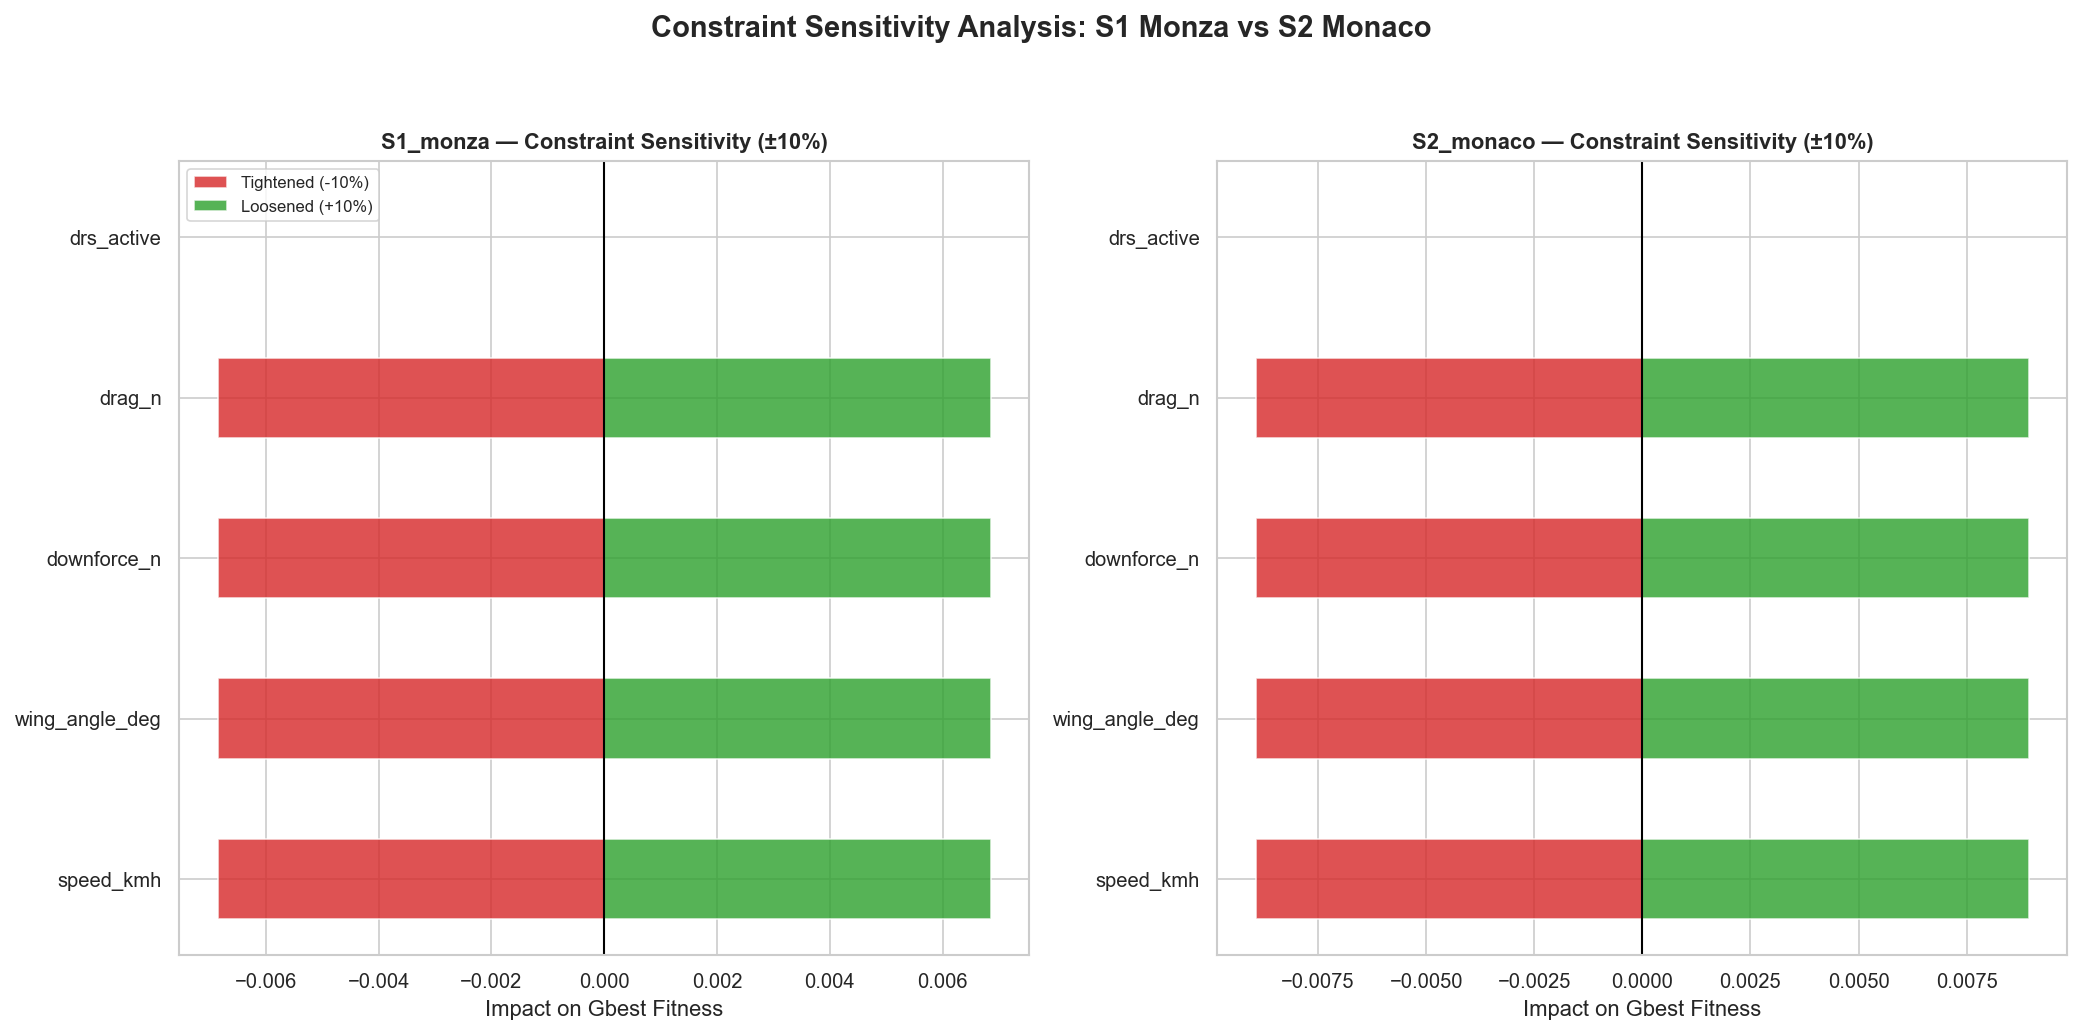
\includegraphics[width=0.78\textwidth]{figures/11_sensitivity_tornado.png}
\caption{四场景约束灵敏度龙卷风图}
\label{fig:tornado}
\end{figure}

图\ref{fig:tornado}展示了各场景下约束变更$\pm 10\%$对最优适应度的影响。
关键发现：
\begin{itemize}
    \item S1 Monza：速度下界（speed\_lb）是唯一敏感约束
        （影响幅度0.045），
        降低速度下限可提升适应度；
    \item S2 Monaco：翼角下界（wing\_lb，0.017）和下压力下界（0.009）
        是主要约束瓶颈；
    \item S3均衡：四约束灵敏度均匀（0.007--0.015），
        无单一瓶颈；
    \item S4湿地：翼角上界最敏感（0.011），
        但放宽上界反而降低适应度——
        OOD区域高翼角导致模型不确定性增大，
        $\lambda\sigma(x)$项产生惩罚。
\end{itemize}

\subsection{加权多目标收敛分析}

\begin{figure}[H]
\centering
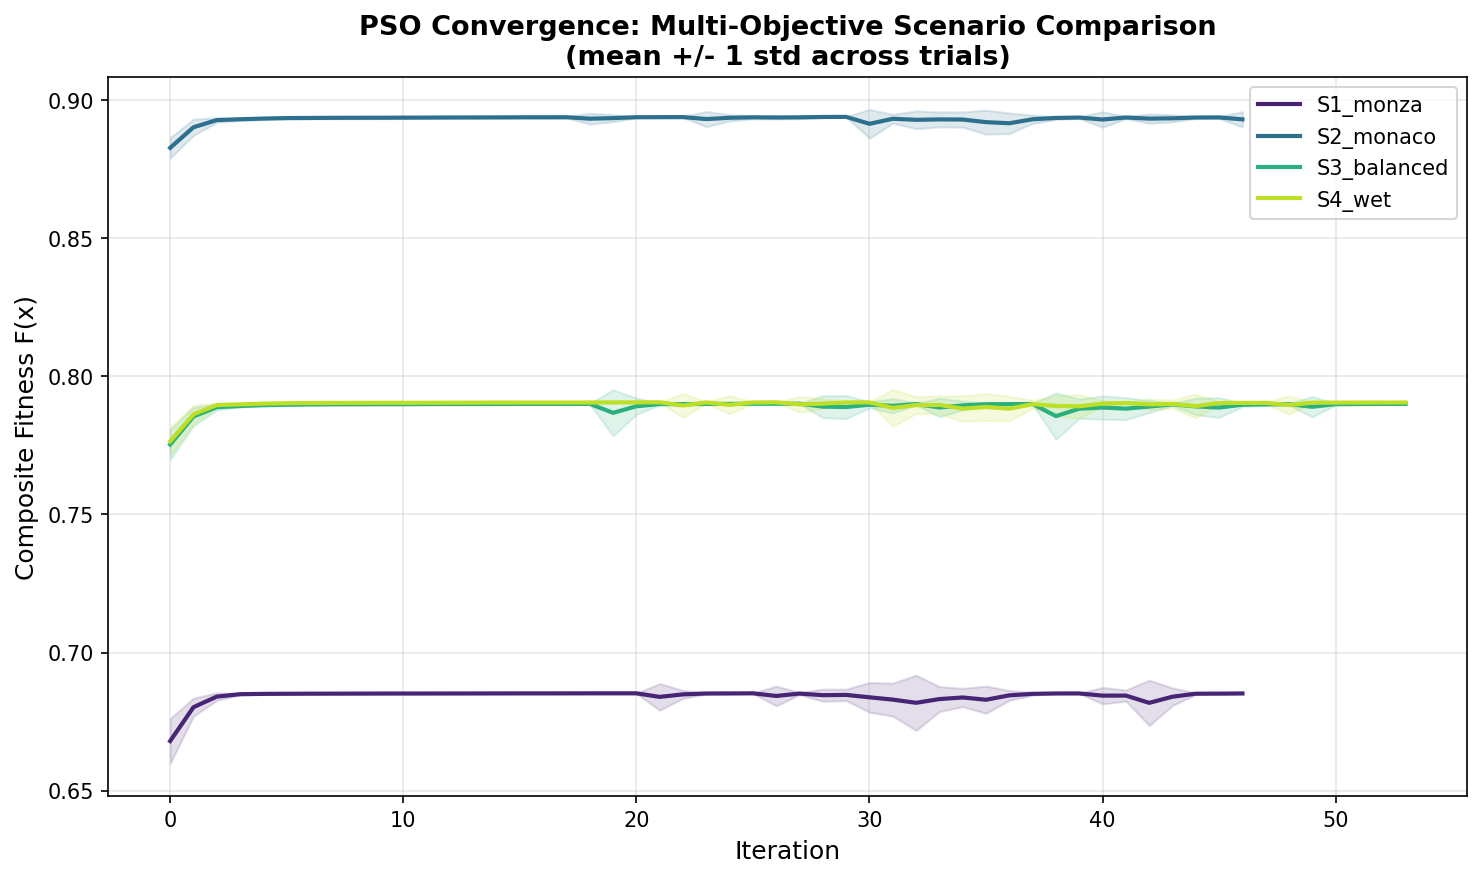
\includegraphics[width=0.78\textwidth]{figures/convergence_multiobj.png}
\caption{多目标PSO收敛曲线（四场景对比）}
\label{fig:multiobj_conv}
\end{figure}

图\ref{fig:multiobj_conv}展示了多目标PSO的复合适应度收敛过程。
与单目标优化（区分度仅0.1\%）形成鲜明对比：
多目标下各场景的复合适应度区间为0.685（S1）$\to$0.894（S2），
差异超23\%，验证了引入效率/功耗竞争性目标后
优化景观被有效"激活"，PSO的价值得以体现。

\subsection{景观多峰性验证}

\begin{figure}[H]
\centering
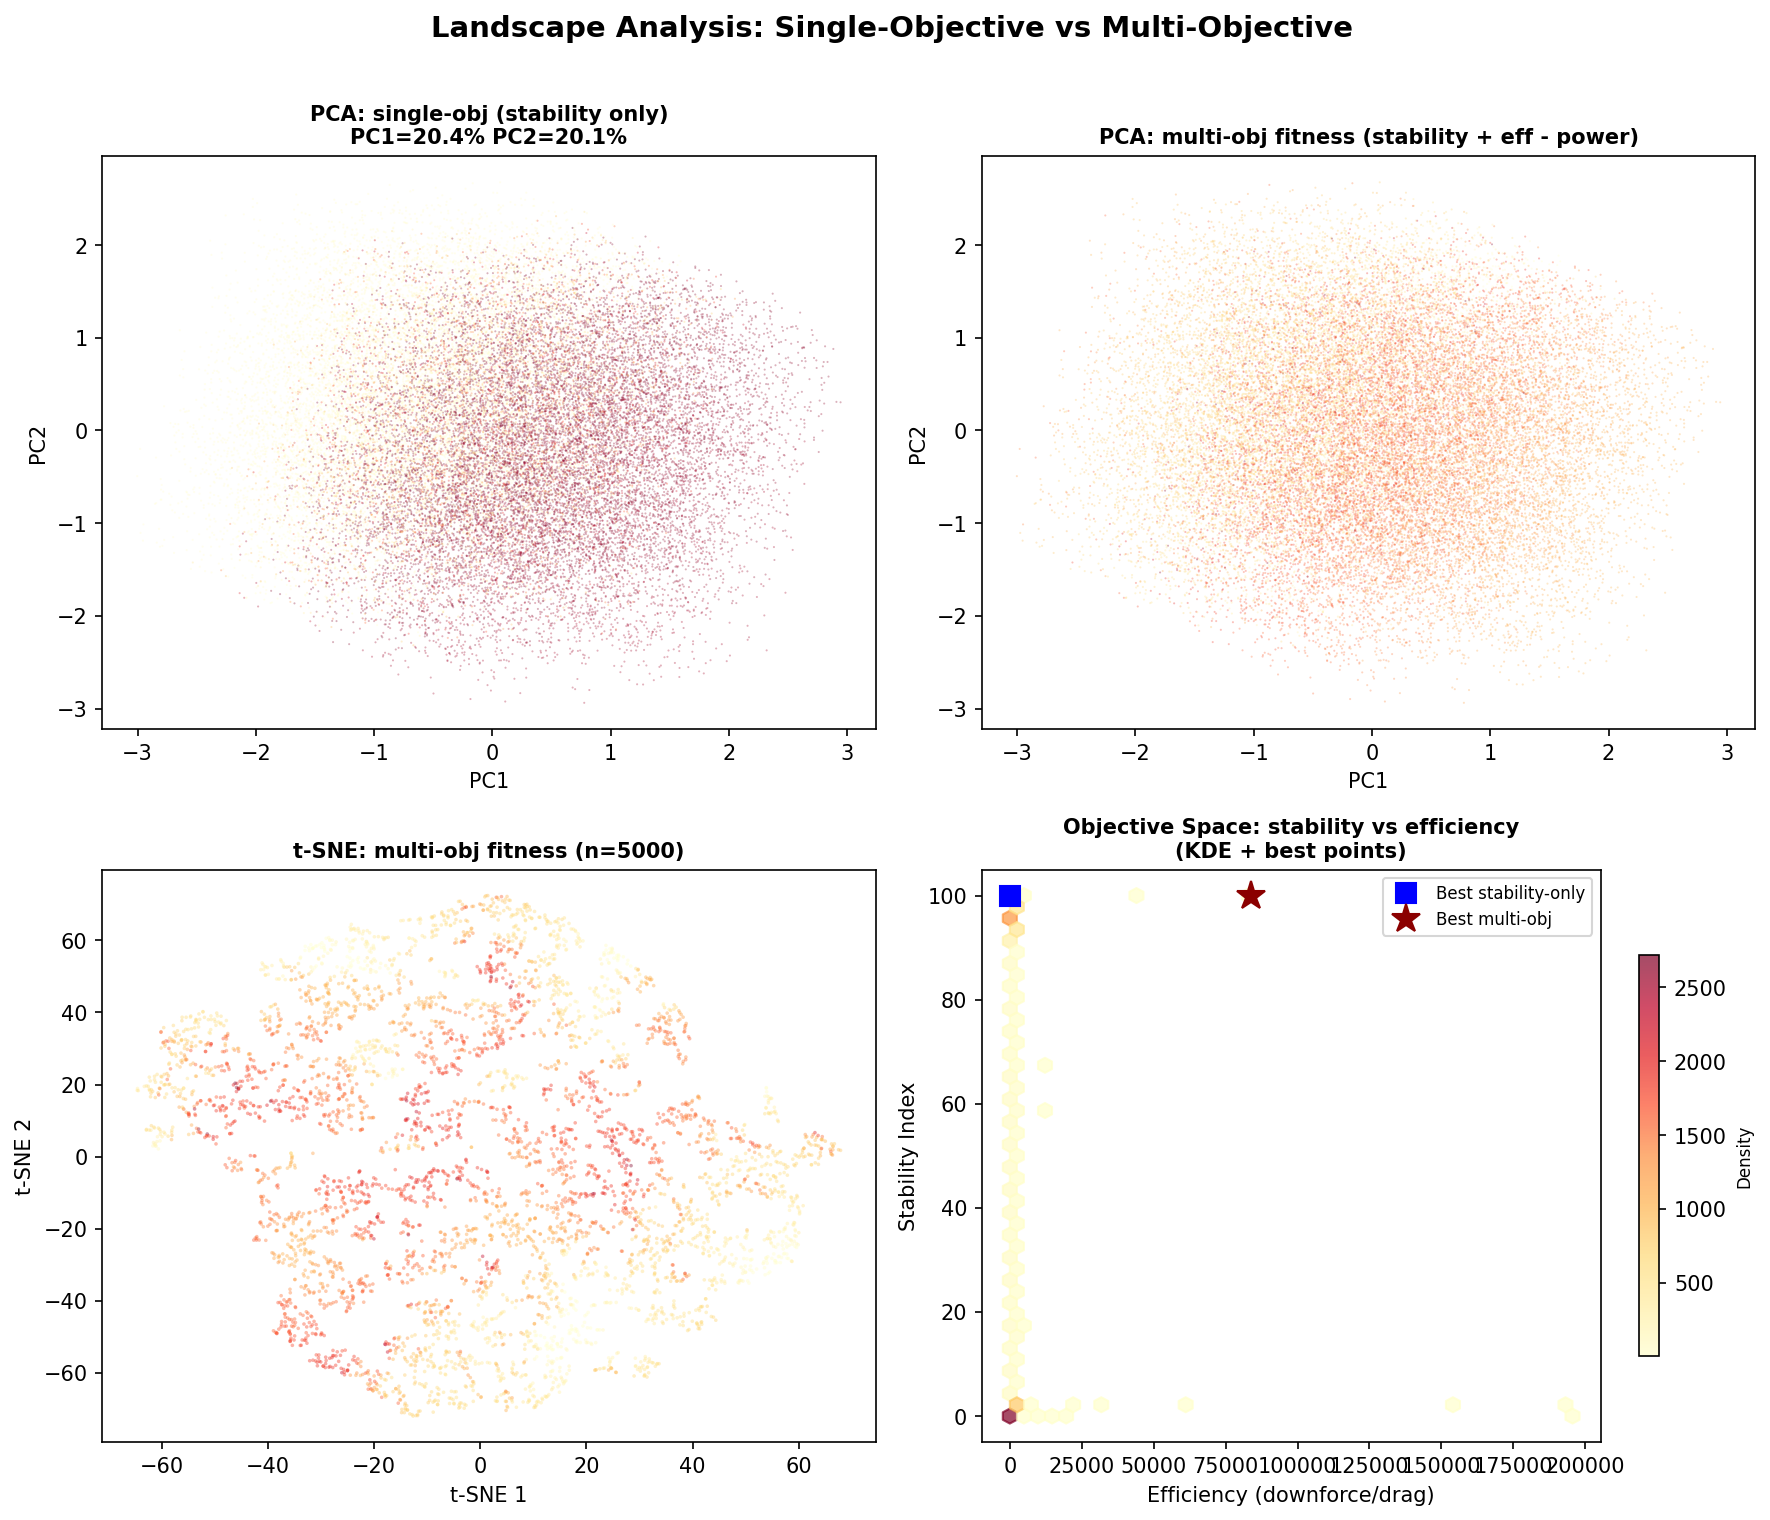
\includegraphics[width=0.80\textwidth]{figures/landscape_multimodality.png}
\caption{优化景观结构分析（PCA + t-SNE + 目标空间热力图）}
\label{fig:landscape}
\end{figure}

图\ref{fig:landscape}通过4个子图验证了多目标优化的景观结构：
\begin{itemize}
    \item 左上（单目标PCA）：一个黄色大簇——景观过平，PSO无意义；
    \item 右上（多目标PCA）：两个分散黄色区——多峰结构出现；
    \item 左下（t-SNE投影）：验证了PCA发现的非单峰结构；
    \item 右下（目标空间KDE）：展示了标量化解的权衡空间分布，
        为PSO的多场景差异化搜索提供了合理的景观基础。
\end{itemize}

\subsection{小结}

多场景优化模块实现了以下成果：
（1）在4组F1赛道工况下完成多目标PSO寻优；
（2）多目标适应度使场景间区分度从0.1\%提升到23\%以上；
（3）SHAP和排列重要性双重验证了在当前特征表示下，
downforce\_n的数值变化与模型预测输出之间存在压倒性的统计关联。
需要指出，SHAP值反映的是特征在模型决策中的相关贡献，
而非物理因果效应——
特别是在downforce\_n与drag\_n共线（$r=0.895$）的场景下，
模型可能将多特征的预测信息集中归因至downforce\_n。
（4）约束灵敏度分析揭示了各场景的设计瓶颈；
（5）景观多峰性验证为PSO的方法论选择提供了量化合理性论证。
